\documentclass[a4paper,10pt,twocolumn]{article}
\usepackage{graphicx}
\usepackage{float}
\floatstyle{ruled}
\newfloat{program}{thp}{lop}
\floatname{program}{Program}

%opening
\title{Virtualization of a Linux File System}
\author{Benjamin Bramble, Zev Weiss}

\begin{document}

\maketitle

\begin{abstract}

\end{abstract}

\section{Introduction}
Recently, the computer science community has taken a renewed interest in virtualization.  
The evolution of true virtual machines, VM's that do not require modifications to the OS, allows for remarkable hypervisors that hide virtualization from the guest machines.  
One such measure of a successful hypervisor is that the performance overhead introduced by virtualization should be small [Xen]. In this paper, we aim to determine the overhead of virtualizing the linux ext 2 file system and make deductions regarding the behind-the-scenes work of the VMM.

First, we sought to find the ideal buffer size for random file access.  
The ideal buffer size would be the maximum size before overstepping the page size and incurring a time penelty.
The easiest way to determine this amount is to conduct reads of various sizes and note the time pattern discrepencies.
In the case of our real and virtual machines, we found that 4KB was the ideal buffer size perfectly matching up with the page size.

The second area researched focused on the amount of data prefetched by the file system during a sequential read of a large file.
To determine the readahead, we had to force a prefetch and conduct various reads at various offsets until the time differential between data stored in the cache and data fetched from memory became clear.
Both the real machine and the virtual machine had 128KB of prefetching.
The interesting aspect of this section is the high level of variance in the VM's reads from memory in comparison to the real machine.
This indicates a fair amount of work conducted by the VMM that was not always consistant. 


\section{Methodology}
\paragraph{System}
\paragraph{Timer} 
\paragraph{Random File Access Buffer}

\paragraph{Sequential Read Prefetch}
\paragraph{File System Cache}
\paragraph{Inode Pointers}
\section{Results}
\paragraph{Random File Access Buffer}
Blah
\begin{program}
  \begin{verbatim}
fd=open(name,RDWR|CREAT,S_IRWXU)
for (i=0;i<=10*1024;i+1024)
   drop_cache   
   offset=lseek(fd,0,SEEK_SET)       
   clock_gettime(Monotonic, start_time)
   read(fd,buf,i)
   clock_gettime(Monotonic, end_time)
   store(i,end_time-start_time)    
close(fd)
\end{verbatim}
  \caption{Pseudo Code for Ideal Buffer Size}
\end{program}

%\begin{figure}[htb]
%\centering
%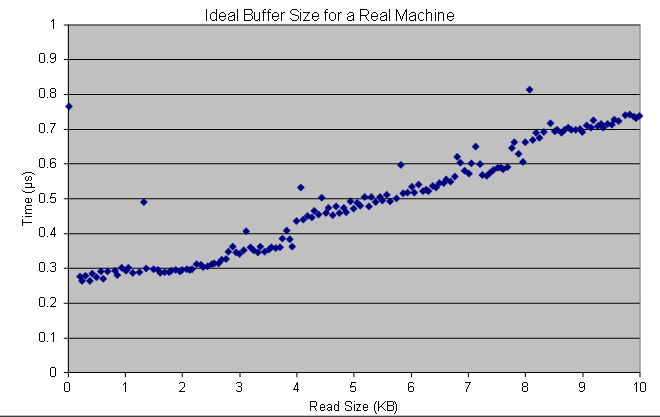
\includegraphics[bb=100 00 300 330,scale=0.5]{buffer_real.png}
%\caption{Ideal Buffer Size for a Real Machine Results}
%\label{fig:awesome_image}
%\end{figure}
%
%\begin{figure}[htb]
%\centering
%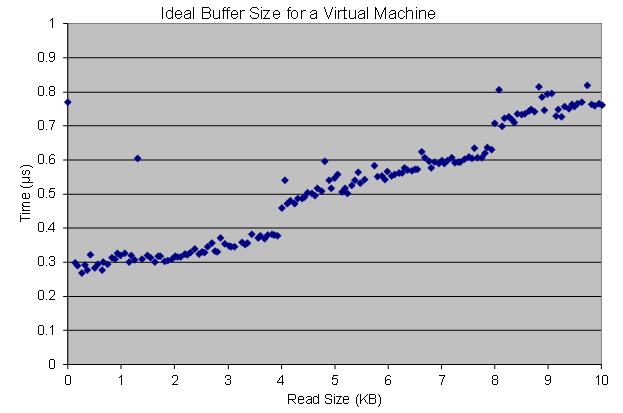
\includegraphics[bb=100 00 300 330,scale=0.5]{buffer_vir.png}
%\caption{Ideal Buffer Size for a Virtual Machine Results}
%\label{fig:awesome_image}
%\end{figure}

\paragraph{Sequential Read Prefetch}
Blah
\begin{program}
  \begin{verbatim}
fd=open(name,RDWR|CREAT,S_IRWXU)
for (i=1024*750;i>=0;i-1024)
   drop_cache   
   pread(fd,buf,50*1024,0)
   lseek(fd,i,seekset)       
   clock_gettime(Monotonic, start_time)
   read(fd,buf,1)
   clock_gettime(Monotonic, end_time)
   store(i,end_time-start_time)    
close(fd)
\end{verbatim}
  \caption{Pseudo Code for Sequential Read Prefetch}
\end{program}

%\begin{figure}[htb]
%\centering
%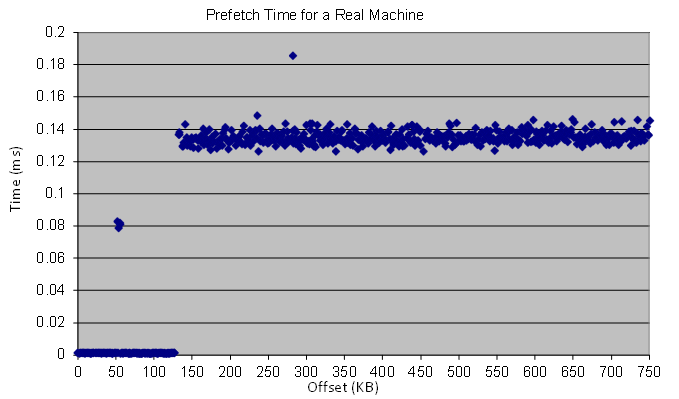
\includegraphics[bb=100 00 300 330,scale=0.5]{prefetch_real.png}
%\caption{Prefetch Size for a Real Machine Results}
%\label{fig:awesome_image}
%\end{figure}
%
%\begin{figure}[htb]
%\centering
%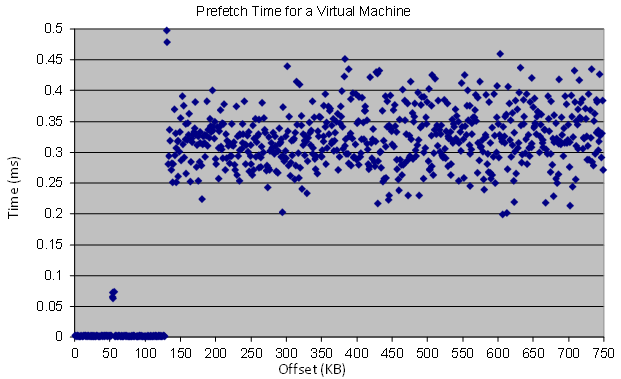
\includegraphics[bb=100 00 300 330,scale=0.5]{prefetch_vir.png}
%\caption{Prefetch Size for a Virtual Machine Results}
%\label{fig:awesome_image}
%\end{figure}


\paragraph{File System Cache}
\paragraph{Inode Pointers}
\section{Conclusion}
\bibliographystyle{plain}
\bibliography{mini_project}
\end{document}
